\chapter{Diseño e implementación} % Main chapter title

\label{Chapter3} % Change X to a consecutive number; for referencing this chapter elsewhere, use \ref{ChapterX}

\definecolor{mygreen}{rgb}{0,0.6,0}
\definecolor{mygray}{rgb}{0.5,0.5,0.5}
\definecolor{mymauve}{rgb}{0.58,0,0.82}

%%%%%%%%%%%%%%%%%%%%%%%%%%%%%%%%%%%%%%%%%%%%%%%%%%%%%%%%%%%%%%%%%%%%%%%%%%%%%
% parámetros para configurar el formato del código en los entornos lstlisting
%%%%%%%%%%%%%%%%%%%%%%%%%%%%%%%%%%%%%%%%%%%%%%%%%%%%%%%%%%%%%%%%%%%%%%%%%%%%%
\lstset{ %
  backgroundcolor=\color{white},   % choose the background color; you must add \usepackage{color} or \usepackage{xcolor}
  basicstyle=\footnotesize,        % the size of the fonts that are used for the code
  breakatwhitespace=false,         % sets if automatic breaks should only happen at whitespace
  breaklines=true,                 % sets automatic line breaking
  captionpos=b,                    % sets the caption-position to bottom
  commentstyle=\color{mygreen},    % comment style
  deletekeywords={...},            % if you want to delete keywords from the given language
  %escapeinside={\%*}{*)},          % if you want to add LaTeX within your code
  %extendedchars=true,              % lets you use non-ASCII characters; for 8-bits encodings only, does not work with UTF-8
  %frame=single,	                % adds a frame around the code
  keepspaces=true,                 % keeps spaces in text, useful for keeping indentation of code (possibly needs columns=flexible)
  keywordstyle=\color{blue},       % keyword style
  language=[ANSI]C,                % the language of the code
  %otherkeywords={*,...},           % if you want to add more keywords to the set
  numbers=left,                    % where to put the line-numbers; possible values are (none, left, right)
  numbersep=5pt,                   % how far the line-numbers are from the code
  numberstyle=\tiny\color{mygray}, % the style that is used for the line-numbers
  rulecolor=\color{black},         % if not set, the frame-color may be changed on line-breaks within not-black text (e.g. comments (green here))
  showspaces=false,                % show spaces everywhere adding particular underscores; it overrides 'showstringspaces'
  showstringspaces=false,          % underline spaces within strings only
  showtabs=false,                  % show tabs within strings adding particular underscores
  stepnumber=1,                    % the step between two line-numbers. If it's 1, each line will be numbered
  stringstyle=\color{mymauve},     % string literal style
  tabsize=2,	                   % sets default tabsize to 2 spaces
  title=\lstname,                  % show the filename of files included with \lstinputlisting; also try caption instead of title
  morecomment=[s]{/*}{*/}
}


%----------------------------------------------------------------------------------------
%	SECTION 1
%----------------------------------------------------------------------------------------
\section{Arquitectura del sistema embebido}
 
\section{Selección de componentes}

\section{Desarrollo de software}

INDICAR QUE EL SOFTWARE SE DESARROLLO PRIMERO EN PLACA DE DESARROLLO Y DESPUES SE IMPLEMENTO

\subsection{Driver CAN}

\subsection{Interfaz HMI}

\subsection{Interfaz UART-USB}

\section{Modificaciones firmware SN-17}

\section{Desarrollo de Hardware}

Para el desarrollo del hardware se utilizó el software de diseño Altium Designer\footnote{\url{https://www.altium.com/}} y se eligió como fabricante a PCBWING\footnote{\url{https://www.pcbwing.com/}} que es una empresa con la que trabaja comúnmente Cambre ICyFSA. Se tomó, como punto de partida, las capacidades técnicas de este fabricante.

Se decidió hacer una placa de 4 capas, con dimensiones menores a 100 x 100 mm. Esto se debe a que el fabricante ofrece precios más económicos para estas especificaciones y se consideró que no imponen restricciones importantes el diseño requerido.

Previo al comienzo del desarrollo del circuito esquemático, se recopiló la información de todos los componentes seleccionados y se cargaron sus pinouts, footprints y modelos 3D. Se seleccionaron, para las conexiones externas, los conectores COMBICON con tornillo y los conectores XH para las conexiones internas del sistema.

Una vez tomadas estas decisiones, el primer paso del diseño fue determinar los subcircuitos del sistema. Estos son:
\begin{itemize}
	\item Microcontrolador
	\item Regulador de tensión	
	\item Interfaz CAN
	\item Entradas discretas
	\item Salidas discretas
	\item Interfaz UART-USB
\end{itemize}

Para cada uno de estos subcircuitos se armó un dibujo esquemático. En la Figura \ref{fig:esquematico_can} puede verse el correspondiente a la interfaz CAN donde se muestra el \textit{transciever} elegido y sus conexiones. Para cada uno de los componentes principales del sistema, se siguieron las recomendaciones indicadas en la hoja de datos correspondiente. 

\begin{figure}[htbp]
	\centering
	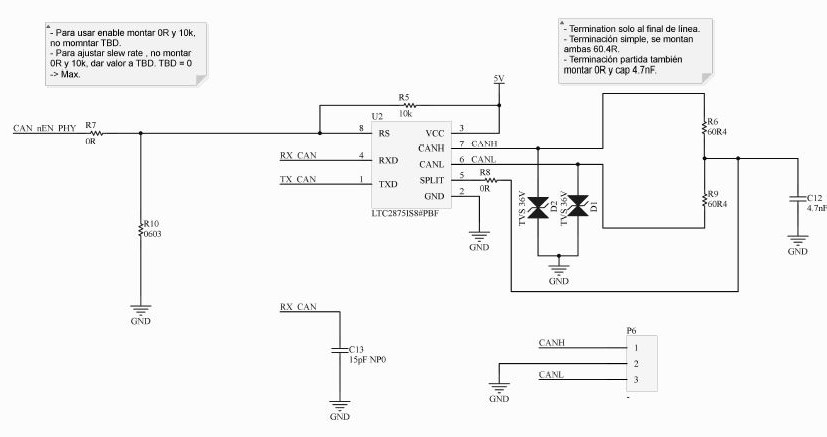
\includegraphics[scale=.6]{./Figures/sch_can.JPG}
	\caption{Esquemático de Interfaz CAN}
	\label{fig:esquematico_can}
\end{figure}

Finalizados los subcircuitos esquemáticos, se procede al desarrollo del PCB. Primero, se determinaron las dimensiones de la plaqueta, manteniendo las restricciones impuestas y asegurando una cómoda posición de todos los componentes, para permitir un ensamble manual. Se llegó a una dimensión final de 100 x 80 mm. 

Para el diseño del PCB se buscó que:
\begin{itemize}
	\item Los subcircuitos quedaran separados.
	\item Los conectores quedaran todos en los extermos de la plaqueta.
	\item Se respetara la aislación eléctrica de las entradas y salidas con el circuito de control.
	\item Las líneas de CAN se mantuvieran lo más cortas y simétricas posibles.
\end{itemize}

La Figura \ref{fig:render_pcb} muestra el render 3D del \textit{PCB} obtenido. En este se pueden ver los detalles mencionados. En la parte superior, se encuentran los circuitos de entradas y salidas industriales, eléctricamente aislados por los optoacopladores y separados del resto del circuito. En la esquina inferior izquierda, se encuentra el regulador de tensión de 5 V. En el centro, el microcontrolador y a la derecha, el circuito de CAN y de USB.

\begin{figure}[htbp]
	\centering
	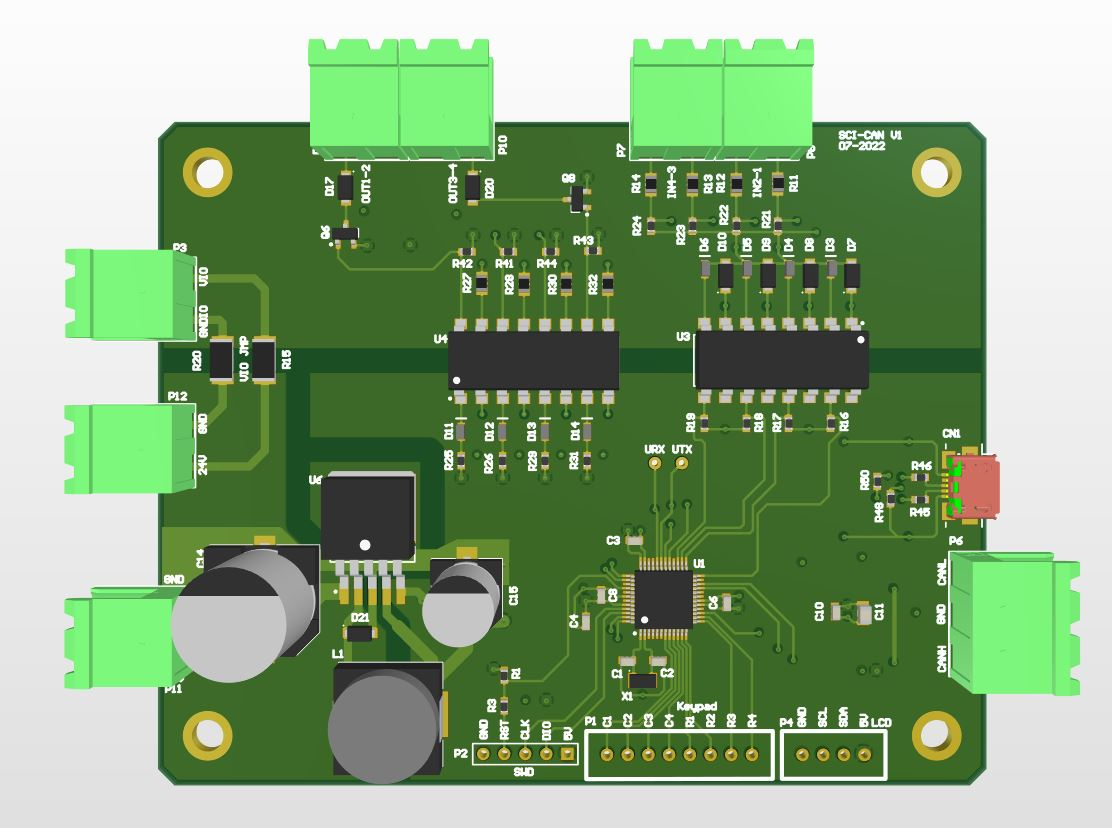
\includegraphics[scale=.5]{./Figures/pcb_sch.JPG}
	\caption{Render del \textit{PCB}}
	\label{fig:render_pcb}
\end{figure}

\section{Desarrollo de gabinete}

Para el desarrollo del gabinete se usó el software de diseño mecánico Autodesk Inventor\footnote{\url{https://www.autodesk.com/products/inventor/overview?term=1-YEAR&tab=subscription}}. Se determinó armar un ensamble que incluya todos los componentes y se lo pensó para poder luego ser impreso en 3D.

Para los componentes comprados, como la pantalla LCD y la matriz de botones, se tomaron los modelos 3D de uso libre de la plataforma GrabCAD\footnote{\url{https://grabcad.com/}}. Estos se verificaron para asegurarse que sus medidas correspondieran con el dispositivo físico adquirido. Por ultimo, el modelo de la plaqueta electrónica desarrollada se exportó desde el software Altium, donde se diseñó.

Una vez obtenidos los modelos de estos componentes, se comenzó con el desarrollo de las distintas piezas que conformarían el gabinete. Como consideraciones del diseño, se priorizó el acceso a los conectores de la plaqueta, para permitir realizar cambios de cableados con poco esfuerzo, pero manteniendo los circuitos protegidos. También, se planteó que el teclado y pantalla estuvieran contiguos, pero con sus conexiones respectivas escondidas dentro del gabinete. Se apuntó a minimizar la cantidad de partes y el tamaño del conjunto. Se tuvo como restricción de tamaño las dimensiones máximas de fabricación de la impresora 3D \textit{Creality Ender-3}\footnote{https://www.creality.com/products/ender-3-3d-printer} (220 x 220 x 250 mm).

En la Figura \ref{fig:ensamble} se presenta una imagen del ensamble tomada de Inventor. Notar que las piezas superiores, donde están la pantalla y el teclado, se muestran transparentes para facilitar la visualización. Como se puede ver, el ensamble consta de 3 componentes: una tapa delantera donde apoyan el display y el teclado, una caja intermedia que encierra a estos y una caja trasera donde se coloca la plaqueta de control. Se decidió por esta forma para permitir una presentación cómoda de los elementos de interfaz, para que el cableado interno quede protegido y para que se tenga fácil acceso a los conectores de la plaqueta, como se mecionó previamente.

\begin{figure}[htbp]
	\centering
	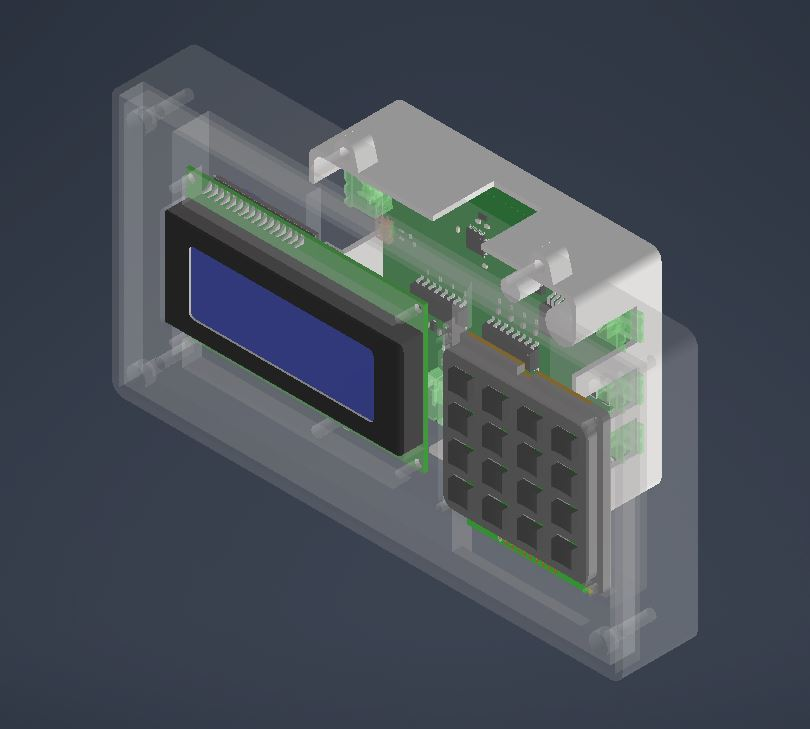
\includegraphics[scale=.6]{./Figures/asm_3d.JPG}
	\caption{Ensamble 3D de gabinete}
	\label{fig:ensamble}
\end{figure}

Una vez cerrado el diseño, se exportó el archivo al programa UltiMaker Cura\footnote{\url{https://ultimaker.com/software/ultimaker-cura}}, donde se generaron los archivos de fabricación para impresión 3D. Se decidió utilizar como material PLA, que es uno de los plásticos más económicos y simples de manipular, y que cuenta con las características mecánicas apropiadas para la aplicación. Luego de fabricado, se forman las roscas en las distintas piezas y se ensambla el conjunto.